\documentclass[10pt,a4paper]{amsart}
\usepackage[margin=19mm]{geometry}
\usepackage{amsmath,amssymb,mathtools}
\usepackage[scr=rsfs,cal=euler]{mathalfa}
\usepackage{xfrac}
\usepackage[unicode,hidelinks,bookmarks=false]{hyperref}
\newcommand{\ie}{i.e.\ }
\newcommand{\cf}{cf.\ }
\newcommand{\resp}{respectively\ }
\newcommand{\Subsection}{\subsection}
\providecommand{\nobreakdash}{\nobreak\hbox{-}}
\setlength{\emergencystretch}{2em}
\multlinegap0pt
\usepackage{tikz}
\usepackage{float}
\usepackage{amssymb}
\newtheorem{theorem}{Theorem}
\title{The zipper condition for $4$-tensors\\ in two-dimensional topological order\\ and the higher relative commutants of a subfactor\\ arising from a commuting square}
\author{Yasuyuki Kawahigashi}
\date{Source: arXiv:2511.10080v2 (CC BY 4.0)}
\begin{document}
\maketitle

\noindent\emph{Source and licence.} The zipper condition for $4$-tensors\\ in two-dimensional topological order\\ and the higher relative commutants of a subfactor\\ arising from a commuting square. Version arXiv:2511.10080v2 (CC BY 4.0), distributed by arXiv under the Creative Commons Attribution 4.0 International licence, http://creativecommons.org/licenses/by/4.0/, as recorded in the arXiv licence metadata for this exact version and shown on the abstract page https://arxiv.org/abs/2511.10080v2. Full licence notice: \texttt{licenses/arxiv-2511.10080-CC-BY-4.0.txt}.\par\smallskip

\noindent\textit{Editorial scope.} Counted unit: the article's theorem zipper (source0.tex lines 1586--1606). The article's complete original proof of it is delivered with it (source0.tex lines 1608--1877, one \texttt{proof} environment of 270 lines). No mathematics is written, repaired or re-derived: the statement and the proof are the article's own lines, in the article's own notation, and no retained line is substituted or re-flowed.  Retained uncounted as the source-local context the proof needs: lines 1103--1137.  Nothing was omitted from any retained span, so the package carries no omission record.  The retained lines cite 1 works, whose entries are transcribed verbatim from the article's own bibliography source in the e-print and delivered with short editorial labels recorded in the item's reference mapping.  The retained lines contain the article's own diagram code, which the wrapper typesets with the standard tikz packages; no image file is delivered and the package declares no asset dependency.  Editorial formatting only, in addition: an AMS \texttt{amsart} preamble that restates the article's own declarations and macros used by the retained lines, namely the environments \texttt{theorem} on separate counters, together with the standard packages those lines need.  The retained environments print in this document as Theorem 1 in order of appearance, whereas the article prints the same items with the numbering of its own full document.  The complete native source of the article as distributed in the arXiv e-print for this exact version is bundled unchanged as \texttt{sources/189014/source0.tex}.
\begin{figure}[H]
\begin{center}
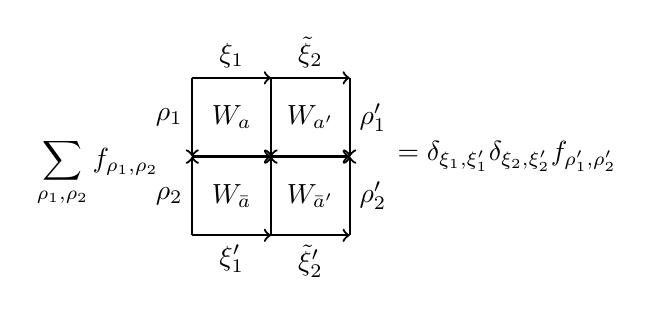
\begin{tikzpicture}
\draw [thick, ->] (3,1)--(4,1);
\draw [thick, ->] (4,1)--(5,1);
\draw [thick, ->] (3,2)--(4,2);
\draw [thick, ->] (4,2)--(5,2);
\draw [thick, ->] (3,3)--(4,3);
\draw [thick, ->] (4,3)--(5,3);
\draw [thick, ->] (3,1)--(3,2);
\draw [thick, ->] (3,3)--(3,2);
\draw [thick, ->] (4,1)--(4,2);
\draw [thick, ->] (4,3)--(4,2);
\draw [thick, ->] (5,1)--(5,2);
\draw [thick, ->] (5,3)--(5,2);
\draw (3.5,2.5)node{$W_a$};
\draw (3.5,1.5)node{$W_{\bar a}$};
\draw (4.5,2.5)node{$W_{a'}$};
\draw (4.5,1.5)node{$W_{\bar a'}$};
\draw (3.5,1)node[below]{$\xi'_1$};
\draw (3.5,3)node[above]{$\xi_1$};
\draw (4.5,1)node[below]{$\tilde\xi'_2$};
\draw (4.5,3)node[above]{$\tilde\xi_2$};
\draw (3,1.5)node[left]{$\rho_2$};
\draw (3,2.5)node[left]{$\rho_1$};
\draw (5,1.5)node[right]{$\rho'_2$};
\draw (5,2.5)node[right]{$\rho'_1$};
\draw (1.8,1.8)node{$\displaystyle\sum_{\rho_1,\rho_2}f_{\rho_1,\rho_2}$};
\draw (7,2)node{$=\delta_{\xi_1,\xi_1'}\delta_{\xi_2,\xi_2'}
f_{\rho'_1,\rho'_2}$};
\end{tikzpicture}
\caption{Flatness of $f$}
\label{flatf}
\end{center}
\end{figure}

\begin{theorem}\label{zipper}
The following are equivalent for a $2$-tensor $F$ and 
the corresponding field $f$ of strings defined as above.

\textnormal{(1) [The half zipper condition]}
There exists another $2$ tensor $\tilde F$ so that
the $2$-tensors $F, \tilde F$ satisfy the intertwining property 
as in Fig.~\ref{intertwine1}.

\textnormal{(2) [The zipper condition]}
The $2$-tensors $F$ satisfies the invariance property 
as in Fig.~\ref{intertwine2}.

\textnormal{(3) [Half flatness]}
There exists another field $\tilde f$ of strings so that we have
the half flatness as in Fig.~\ref{halfflatf}.

\textnormal{(4) [Flatness]}
The field $f$ of strings satisfies
the flatness as in Fig.~\ref{flatf}.
\end{theorem}

\begin{proof}

We first show equivalence of (3) and (4)
Recall that this has been essentially
proved in \cite[pages 563--564]{EK1}, but we give more
details in the current context.
Using the initial connection $W_a$, we apply the
string algebra construction in \cite[Section 11.3]{EK1},
but allow all vertices in $V_0$ to be starting vertices.
We then have a double sequence $\{A_{jk}\}_{j,k=1,2,\dots}$
of finite dimensional $C^*$-algebras and $A_{00}$
is an abelian algebra $\mathbb{C}^{|V_0|}$, where
$|V_0|$ denotes the cardinality of $V_0$.  

We assume (3).  The fields of strings $f$ and $\tilde f$
give the corresponding same elements in the algebras $A_{10}$
and $A_{11}$.  We use the symbol $f$ for this.  
Half flatness implies $f$ commutes with $A_{01}$.
The first horizontal Jones projection $e_1$ commutes with
$A_{10}$, so it commutes with $f$, in particular.  This
means $f$ commutes with $A_{02}$ which is generated by
$A_{01}$ and $e_1$.  This shows $f$ produces another
field of strings $\bar f$ on $\mathcal{G}_1$.  The
argument for $z=z'$ in \cite[Fig.~11.16]{EK1} shows
that the field of strings $\bar f$ is equal to the
field of strings $f$.  This implies (4).

Conversely, we assume (4).  In the same way as the
above argument, we construct string algebras 
$\{A_{jk}\}_{j,k=1,2,\dots}$.  The flatness of
$f$ shows that $f$ gives an element in $A_{10}$ which
commutes with $A_{02}$.  In particular, it commutes with
$A_{01}$, and produces a field $\tilde f$ of strings
satisfying the half flatness condition.

We next prove that (3) implies (1).
We first assume half flatness for $f$ and $\tilde f$.
We define a $2$-tensor $\tilde F$ from $\tilde f$ in
a similar way to the definition of $F$.

\begin{figure}[H]
\begin{center}
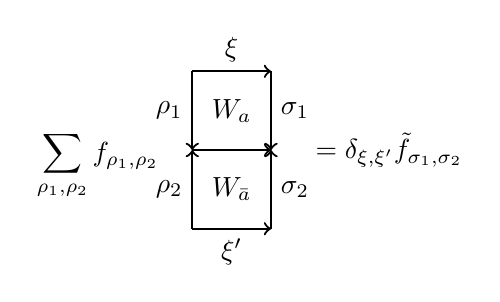
\begin{tikzpicture}
\draw [thick, ->] (3,1)--(4,1);
\draw [thick, ->] (3,2)--(4,2);
\draw [thick, ->] (3,3)--(4,3);
\draw [thick, ->] (3,1)--(3,2);
\draw [thick, ->] (3,3)--(3,2);
\draw [thick, ->] (4,1)--(4,2);
\draw [thick, ->] (4,3)--(4,2);
\draw (3.5,2.5)node{$W_a$};
\draw (3.5,1.5)node{$W_{\bar a}$};
\draw (3.5,1)node[below]{$\xi'$};
\draw (3.5,3)node[above]{$\xi$};
\draw (3,1.5)node[left]{$\rho_2$};
\draw (3,2.5)node[left]{$\rho_1$};
\draw (4,1.5)node[right]{$\sigma_2$};
\draw (4,2.5)node[right]{$\sigma_1$};
\draw (1.8,1.8)node{$\displaystyle\sum_{\rho_1,\rho_2}f_{\rho_1,\rho_2}$};
\draw (5.5,2)node{$=\delta_{\xi,\xi'}\tilde f_{\sigma_1,\sigma_2}$};
\end{tikzpicture}
\caption{Half flatness of $f$}
\label{halfflatf}
\end{center}
\end{figure}

\begin{figure}[H]
\begin{center}
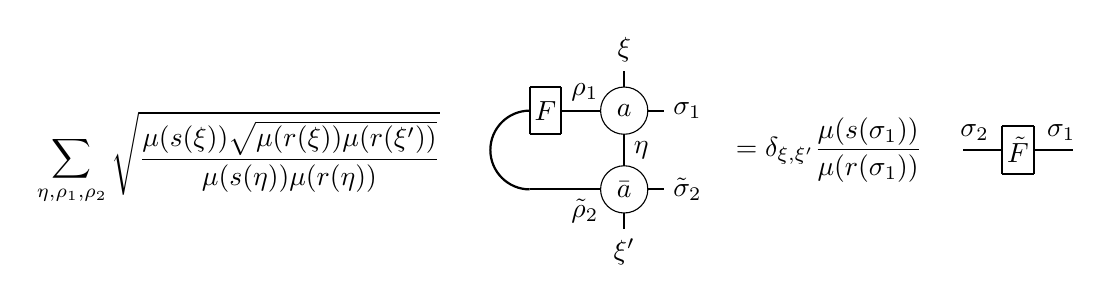
\begin{tikzpicture}
\draw [thick] (8,1)--(8,1.2);
\draw [thick] (8,2)--(8,1.8);
\draw [thick] (6.8,1.5)--(7.7,1.5);
\draw [thick] (8.5,1.5)--(8.3,1.5);
\draw (8,1.5) circle (0.3);
\draw (8,1.5)node{$\bar a$};
\draw [thick] (8,2)--(8,2.2);
\draw [thick] (8,3)--(8,2.8);
\draw [thick] (7.2,2.5)--(7.7,2.5);
\draw [thick] (8.5,2.5)--(8.3,2.5);
\draw (8,2.5) circle (0.3);
\draw (8,2.5)node{$a$};
\draw [thick] (6.8,2.2)--(7.2,2.2);
\draw [thick] (6.8,2.8)--(7.2,2.8);
\draw [thick] (6.8,2.2)--(6.8,2.8);
\draw [thick] (7.2,2.2)--(7.2,2.8);
\draw (7,2.5)node{$F$};
\draw [thick] (6.8,2.5) arc (90:270:0.5);
\draw (7.5,2.5)node[above]{$\rho_1$};
\draw (7.5,1.5)node[below]{$\tilde\rho_2$};
\draw (8.5,1.5)node[right]{$\tilde\sigma_2$};
\draw (8.5,2.5)node[right]{$\sigma_1$};
\draw (8,1)node[below]{$\xi'$};
\draw (8,3)node[above]{$\xi$};
\draw (8,2)node[right]{$\eta$};
\draw (3.1,1.9)node{$\displaystyle\sum_{\eta,\rho_1,\rho_2}
\sqrt{\frac{\mu(s(\xi))\sqrt{\mu(r(\xi))\mu(r(\xi'))}}
{\mu(s(\eta))\mu(r(\eta))}}$};
\draw [thick] (12.8,1.7)--(13.2,1.7);
\draw [thick] (12.8,2.3)--(13.2,2.3);
\draw [thick] (12.8,1.7)--(12.8,2.3);
\draw [thick] (13.2,1.7)--(13.2,2.3);
\draw [thick] (12.8,2)--(12.3,2);
\draw [thick] (13.2,2)--(13.7,2);
\draw (13,2)node{$\tilde F$};
\draw (13.55,2)node[above]{$\sigma_1$};
\draw (12.45,2)node[above]{$\sigma_2$};
\draw (10.6,2)node{$=\delta_{\xi,\xi'}\displaystyle
\frac{\mu(s(\sigma_1))}{\mu(r(\sigma_1))}$};
\end{tikzpicture}
\caption{Half flatness for $F$}
\label{halfflatff}
\end{center}
\end{figure}

We rewrite the coefficient within the summation on the
left-hand side as
\[
\frac{\mu(s(\xi))}{\mu(s(\eta))}
\sqrt{\frac{\sqrt{\mu(r(\xi))\mu(r(\xi'))}\mu(s(\eta))}
{\mu(s(\xi))\mu(r(\eta))}},
\]
and multiply the number in Fig.~\ref{multi} to the numbers on
the both hands sides of Fig.~\ref{halfflatff} and sum them
over $\xi',\sigma_2$.  

\begin{figure}[H]
\begin{center}
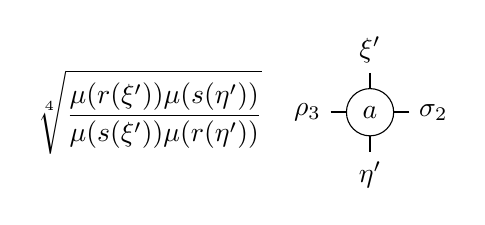
\begin{tikzpicture}
\draw [thick] (3,1)--(3,1.2);
\draw [thick] (3,2)--(3,1.8);
\draw [thick] (2.5,1.5)--(2.7,1.5);
\draw [thick] (3.5,1.5)--(3.3,1.5);
\draw (3,1.5) circle (0.3);
\draw (3,1.5)node{$a$};
\draw (2.5,1.5)node[left]{$\rho_3$};
\draw (3.5,1.5)node[right]{$\sigma_2$};
\draw (3,1)node[below]{$\eta'$};
\draw (3,2)node[above]{$\xi'$};
\draw (0.2,1.5)node{$\displaystyle\sqrt[4]{\frac{\mu(r(\xi'))\mu(s(\eta'))}
{\mu(s(\xi'))\mu(r(\eta'))}}$};
\end{tikzpicture}
\caption{The multiplier}
\label{multi}
\end{center}
\end{figure}

Then by bi-unitarity (2), only the terms for
$\eta=\eta'$ and $\rho_2=\rho_3$ remain, and
we have the identity as in
Fig.~\ref{intertwine1} by dividing the both
hand sides by 
\[
\frac{\mu(r(\sigma_1))}{\mu(s(\sigma_1))}
\displaystyle\sqrt[4]{\frac{\mu(r(\xi))\mu(s(\eta'))}
{\mu(s(\xi))\mu(r(\eta'))}}.
\]
Note that only the term $\xi=\xi'$ remains on
the right hand side due to $\delta_{\xi,\xi'}$.
This proves (1).

Since the above graphical manipulation amounts to
a multiplication of a unitary matrix, we also have
the converse direction.  That is, 
we know that (1) implies (3).

A similar argument to the proof of equivalence of (1)
and (3) shows equivalence of (2) and (4).

\begin{figure}[H]
\begin{center}
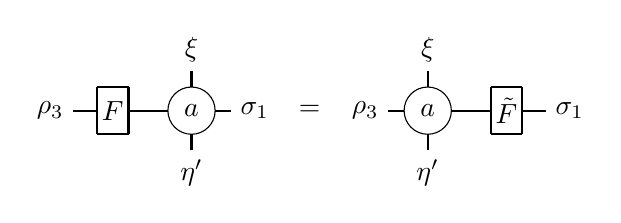
\begin{tikzpicture}
\draw [thick] (2.5,1.5)--(2.5,1.7);
\draw [thick] (2.5,2.5)--(2.5,2.3);
\draw [thick] (1.7,2)--(2.2,2);
\draw [thick] (3,2)--(2.8,2);
\draw (2.5,2) circle (0.3);
\draw (2.5,2)node{$a$};
\draw [thick] (1.3,1.7)--(1.7,1.7);
\draw [thick] (1.3,2.3)--(1.7,2.3);
\draw [thick] (1.3,1.7)--(1.3,2.3);
\draw [thick] (1.7,1.7)--(1.7,2.3);
\draw [thick] (1.3,2)--(1,2);
\draw (1.5,2)node{$F$};
\draw (1,2)node[left]{$\rho_3$};
\draw (3,2)node[right]{$\sigma_1$};
\draw (2.5,2.5)node[above]{$\xi$};
\draw (2.5,1.5)node[below]{$\eta'$};
\draw (4,2)node{$=$};
\draw [thick] (5.5,1.5)--(5.5,1.7);
\draw [thick] (5.5,2.5)--(5.5,2.3);
\draw [thick] (5,2)--(5.2,2);
\draw [thick] (6.3,2)--(5.8,2);
\draw (5.5,2) circle (0.3);
\draw (5.5,2)node{$a$};
\draw [thick] (6.3,1.7)--(6.7,1.7);
\draw [thick] (6.3,2.3)--(6.7,2.3);
\draw [thick] (6.3,1.7)--(6.3,2.3);
\draw [thick] (6.7,1.7)--(6.7,2.3);
\draw [thick] (6.7,2)--(7,2);
\draw (6.5,2)node{$\tilde F$};
\draw (5,2)node[left]{$\rho_3$};
\draw (7,2)node[right]{$\sigma_1$};
\draw (5.5,2.5)node[above]{$\xi$};
\draw (5.5,1.5)node[below]{$\eta'$};
\end{tikzpicture}
\caption{Intertwining property for $F, \tilde F$}
\label{intertwine1}
\end{center}
\end{figure}




\begin{figure}[H]
\begin{center}
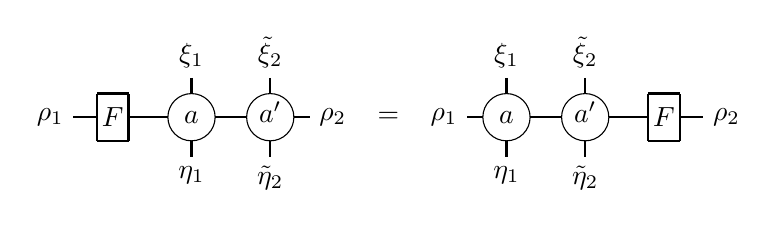
\begin{tikzpicture}
\draw [thick] (2.5,1.5)--(2.5,1.7);
\draw [thick] (2.5,2.5)--(2.5,2.3);
\draw [thick] (3.5,1.5)--(3.5,1.7);
\draw [thick] (3.5,2.5)--(3.5,2.3);
\draw [thick] (1.7,2)--(2.2,2);
\draw [thick] (2.8,2)--(3.2,2);
\draw [thick] (3.8,2)--(4,2);
\draw (2.5,2) circle (0.3);
\draw (2.5,2)node{$a$};
\draw (3.5,2) circle (0.3);
\draw (3.5,2.07)node{$a'$};
\draw [thick] (1.3,1.7)--(1.7,1.7);
\draw [thick] (1.3,2.3)--(1.7,2.3);
\draw [thick] (1.3,1.7)--(1.3,2.3);
\draw [thick] (1.7,1.7)--(1.7,2.3);
\draw [thick] (1.3,2)--(1,2);
\draw (1.5,2)node{$F$};
\draw (1,2)node[left]{$\rho_1$};
\draw (4,2)node[right]{$\rho_2$};
\draw (2.5,2.5)node[above]{$\xi_1$};
\draw (3.5,2.5)node[above]{$\tilde\xi_2$};
\draw (2.5,1.5)node[below]{$\eta_1$};
\draw (3.5,1.5)node[below]{$\tilde\eta_2$};
\draw (5,2)node{$=$};
\draw [thick] (6.5,1.5)--(6.5,1.7);
\draw [thick] (6.5,2.5)--(6.5,2.3);
\draw [thick] (7.5,1.5)--(7.5,1.7);
\draw [thick] (7.5,2.5)--(7.5,2.3);
\draw [thick] (6,2)--(6.2,2);
\draw [thick] (6.8,2)--(7.2,2);
\draw [thick] (7.8,2)--(8.3,2);
\draw [thick] (8.7,2)--(9,2);
\draw (6.5,2) circle (0.3);
\draw (7.5,2) circle (0.3);
\draw (6.5,2)node{$a$};
\draw (7.5,2.07)node{$a'$};
\draw [thick] (8.3,1.7)--(8.7,1.7);
\draw [thick] (8.3,2.3)--(8.7,2.3);
\draw [thick] (8.3,1.7)--(8.3,2.3);
\draw [thick] (8.7,1.7)--(8.7,2.3);
\draw (8.5,2)node{$F$};
\draw (6,2)node[left]{$\rho_1$};
\draw (9,2)node[right]{$\rho_2$};
\draw (6.5,2.5)node[above]{$\xi_1$};
\draw (6.5,1.5)node[below]{$\eta_1$};
\draw (7.5,2.5)node[above]{$\tilde\xi_2$};
\draw (7.5,1.5)node[below]{$\tilde\eta_2$};
\end{tikzpicture}
\caption{Intertwining property for $F$}
\label{intertwine2}
\end{center}
\end{figure}

\end{proof}

\begin{thebibliography}{99}
\bibitem[EK1]{EK1} D. E. Evans and Y. Kawahigashi, ``Quantum Symmetries on Operator Algebras'', Oxford University Press, Oxford (1998).
\end{thebibliography}
\end{document}
